\section{Embedded audio Hardware}

\begin{frame}{Anatomy}
  \begin{center}
    \includegraphics[width=\textwidth]{slides/audio-hardware/anatomy.pdf}\\
    {\em Example of an embedded system sound card}
  \end{center}
\end{frame}

\subsection{CODECs}

\begin{frame}{CODECs}
  \begin{itemize}
  \item A CODEC is a device that COdes and DECodes audio samples.
  \item It integrates an analog-to-digital converter (ADC) and a
    digital-to-analog converter (DAC) into a single chip.
  \item It converts a voltage signal from an analog input (e.g.
    microphone) to a sequence of samples or converts a stream of
    samples to a voltage for an analog output (e.g. speaker driver).
  \item It also has one or multiple digital audio interfaces (DAI) to
    transfer samples to or from a microcontroller or microprocessor.
  \item Usually an extra digital bus is used for configuration
  \end{itemize}
\end{frame}

\begin{frame}[fragile]{Digital audio interface - signals}
  The CODEC DAI is a synchronous serial bus. A common PCM interface is
  represented here:
  \begin{center}
    \includegraphics[height=0.4\textheight]{slides/audio-hardware/i2s.pdf}\\
  \end{center}
\end{frame}


\begin{frame}[fragile]{Digital audio interface - signals}
  \begin{itemize}
  \item The PCM DAI uses two clocks: the bit clock and the frame clock.
  \begin{itemize}
  \item The bit clock is usually referred to as BCK or BCLK
  \item The frame clock is often called FCLK/FSCK/FSCLK, LRCK/LRCLK
    (Left Right clock) or WCLK (word clock). Its rate is the sample
    rate also called Fs.
  \item The relationship between BCK and FSCK is: bck = fsck ∗
    Nchannels ∗ BitDepth
  \end{itemize}
  \item It also has one or multiple data lines.
  \end{itemize}
\end{frame}

\begin{frame}[fragile]{Digital audio interface - Data}
  \begin{itemize}
  \item Codecs may have multiple data in or data out lines, one line
    per channel pair.
  \item Codecs may also have multiple DAI, one full interface for data
    in and one for data out.
  \end{itemize}
  \begin{columns}
    \column{0.5\textwidth}
    e.g.
    \href{https://www.analog.com/media/en/technical-documentation/data-sheets/AD1937.pdf}
    {AD1937} has:
    \begin{itemize}
    \item 8 DACs in 4 pairs, 4 ADCs in 2 pairs
    \item clocks for data-in: DBCLK, DLRCLK
    \item 4 data-in lines (DSDATA[1-4])
    \item clocks for data-out: ABCLK, ALRCLK
    \item 2 data-out lines (ASDATA[1-4])
    \end{itemize}
    \column{0.5\textwidth}
    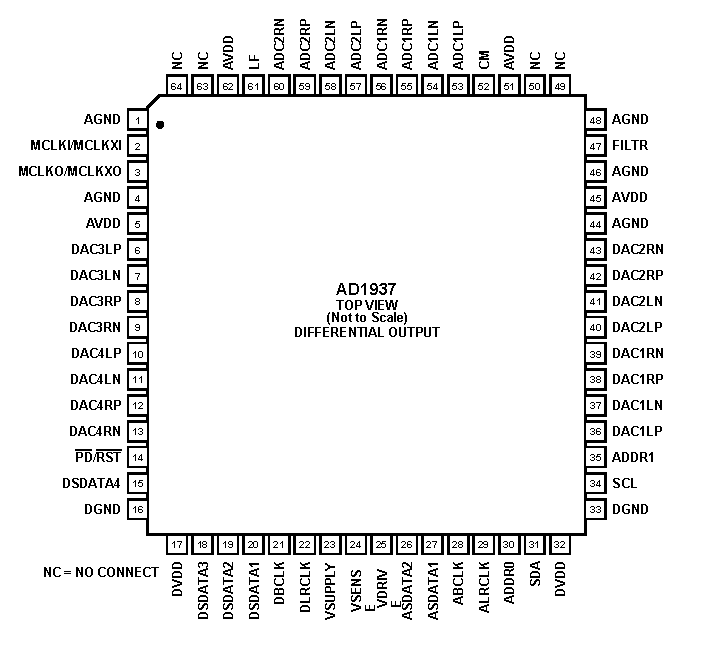
\includegraphics[width=\textwidth]{slides/audio-hardware/ad1937.pdf}\\
  \end{columns}
\end{frame}

\begin{frame}{MCLK}
  \begin{itemize}
  \item MCLK is the codec clock. It is sometimes referred as the
    system clock. The IC needs it to be working.
  \item Some codecs will also require it to be able to use the
    control interface.
  \item Can be provided by the SoC when it has suitable clocks or a
    crystal.
  \item Some codecs are able to use BCLK or LRCLK as their clock,
    making MCLK optional.
  \item usually the codecs will expect MCLK to be a multiple of BCLK.
    Usually specified as a multiple of Fs.
  \end{itemize}
\end{frame}

\subsection{SoC Digital Audio Interface}

\begin{frame}{SoC}
  \begin{itemize}
  \item The SoC also has a dedicated synchronous serial interface.
  \item Some are generic serial interfaces others are dedicated to audio
    formats.
  \item It has a DMA controller or a peripheral DMA controller (PDC)
    able to copy samples from memory to the serial interface registers
    or FIFO.
  \item It quite often also has dedicated multimedia (audio/video) clocks.
  \item Examples: Atmel SSC, NXP SSI, NXP SAI, TI McASP
  \item Some SoCs have a separate SPDIF controller
  \item Some SoCs (Allwinner A33, Atmel SAMA5D2) have the codec and
    the amplifier on the SoC itself so the sound card is completely on
    the SoC.
  \end{itemize}
\end{frame}

\subsection{Digital formats}

\begin{frame}{Digital formats - Left Justified}
    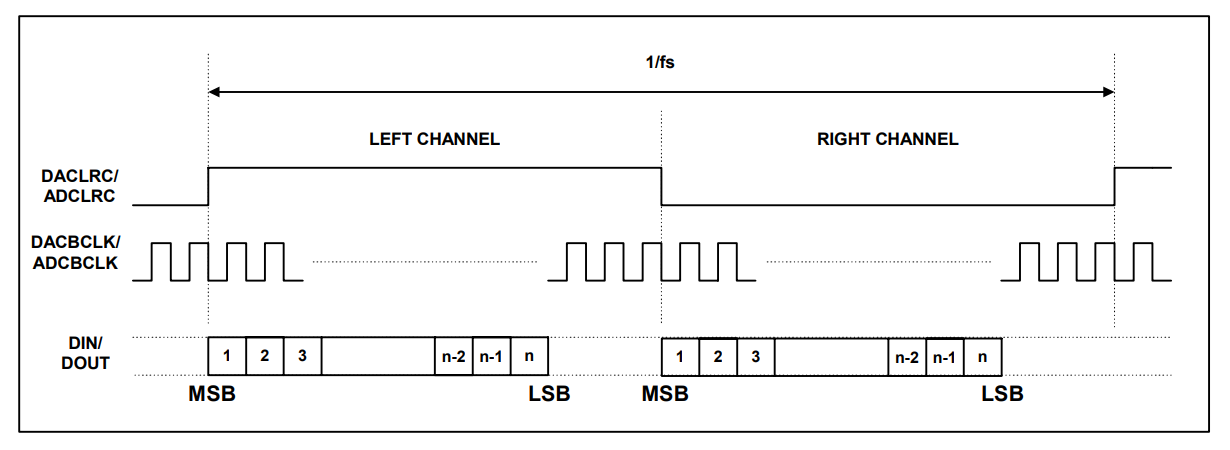
\includegraphics[width=\textwidth]{slides/audio-hardware/LJ.png}\\
\end{frame}

\begin{frame}{Digital formats - Right Justified}
    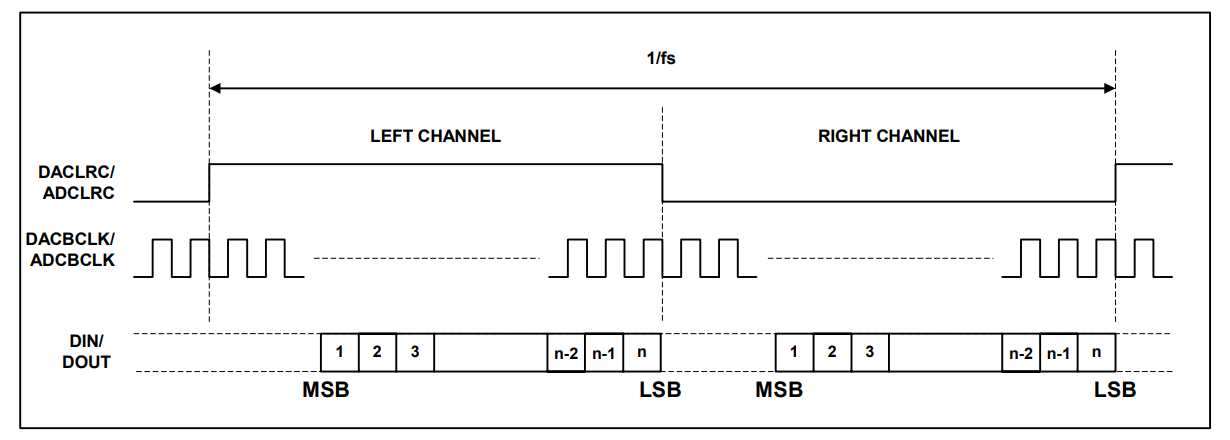
\includegraphics[width=\textwidth]{slides/audio-hardware/RJ.png}\\
\end{frame}

\begin{frame}{Digital formats - I2S}
    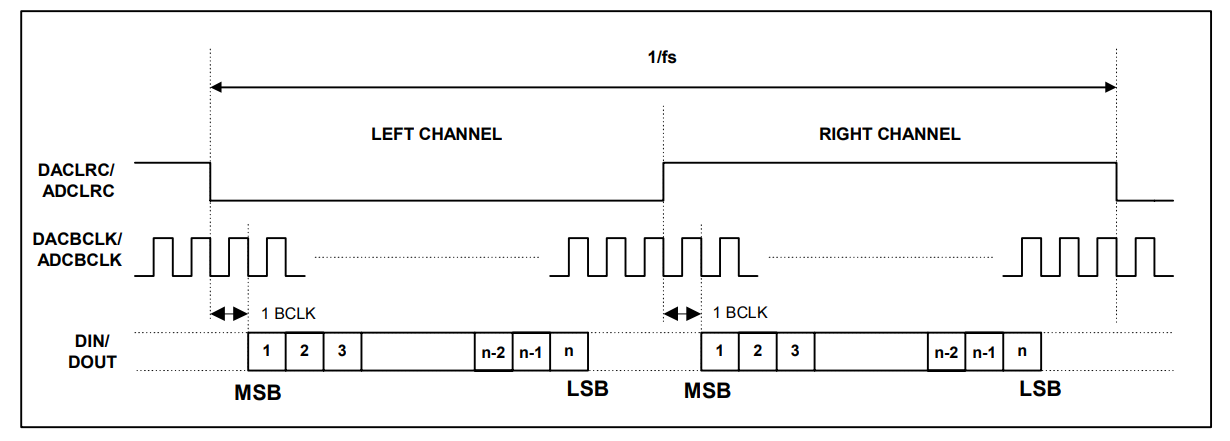
\includegraphics[width=\textwidth]{slides/audio-hardware/I2S.png}\\
\end{frame}

\begin{frame}{Digital formats - DSP A}
    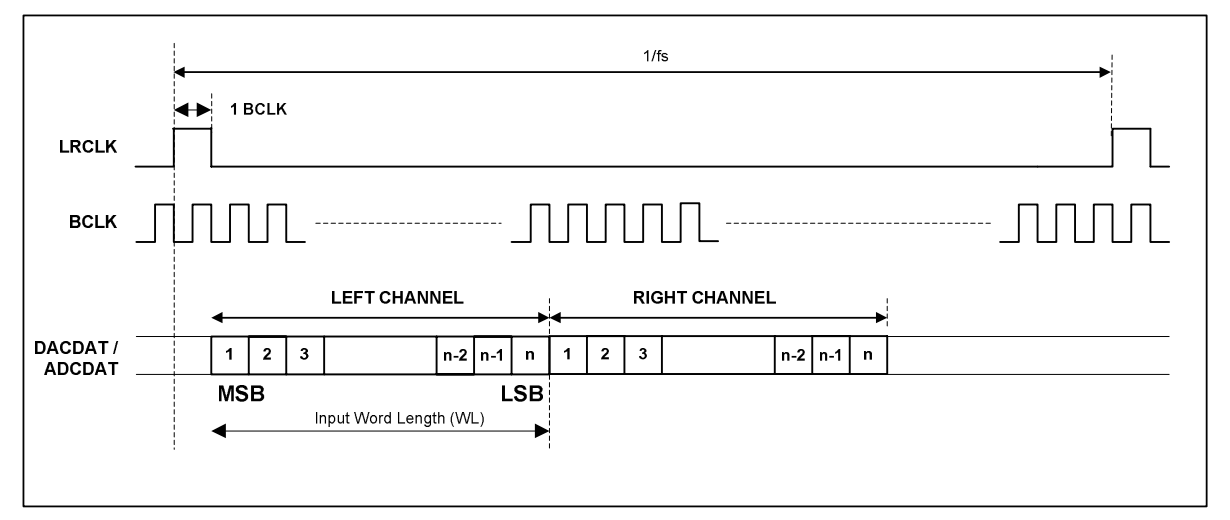
\includegraphics[width=\textwidth]{slides/audio-hardware/DSP_A.png}\\
\end{frame}

\begin{frame}{Digital formats - DSP B}
    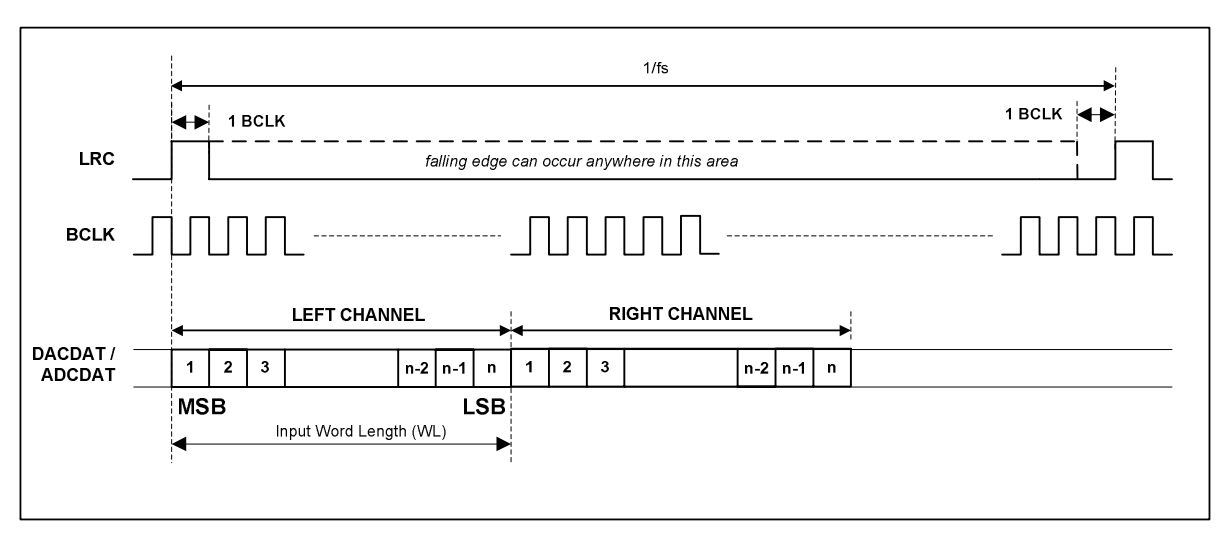
\includegraphics[width=\textwidth]{slides/audio-hardware/DSP_B.png}\\
\end{frame}

\begin{frame}{Digital formats - TDM}
    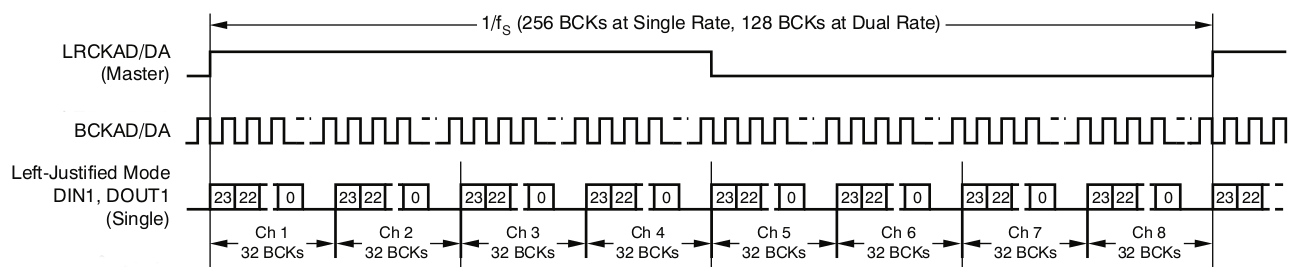
\includegraphics[width=\textwidth]{slides/audio-hardware/TDM.png}\\
\end{frame}

\begin{frame}{Digital formats - AC-link}
  AC97 uses TDM slots. Slot 0 is 16bit wide and is the tag. Then
  twelve 20bit wide slots are used to transmit data.
  \begin{center}
    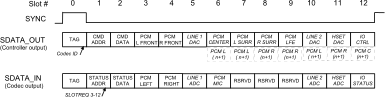
\includegraphics[height=0.3\textheight]{slides/audio-hardware/ac97.pdf}\\
  \end{center}
  \begin{center}
    
\includegraphics[height=0.3\textheight]{slides/audio-hardware/ac97_phases.pdf}\\
  \end{center}
\end{frame}

\begin{frame}{Digital formats - PDM}
  There is another, less common interface, using Pulse Density
  Modulation. It has two signals per channels, clock and data. Data
  has only one bit.\\
  \begin{center}
    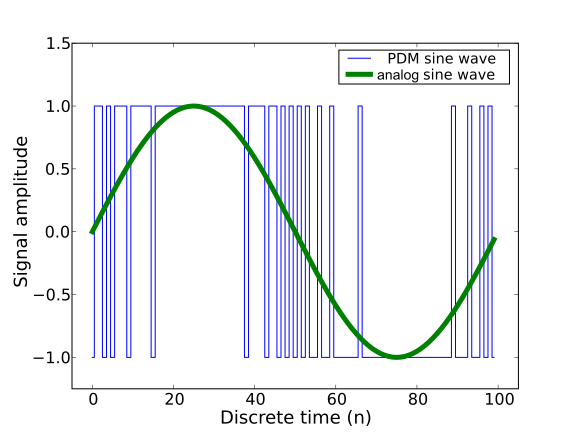
\includegraphics[height=0.8\textheight]{slides/audio-hardware/PDM.pdf}\\
  \end{center}
\end{frame}

\begin{frame}{Digital formats - S/PDIF or IEC 60958}
  S/PDIF uses only one wire. Data is encoded using BMC (Biphase Mark
  Code), also known as differential Manchester encoding. Its clock is
  then twice the bitrate.
  \begin{center}
    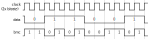
\includegraphics[height=0.2\textheight]{slides/audio-hardware/BMC.pdf}\\
  \end{center}
  Blocks of 192 frames are transmitted, each frame consisting of two
  subframes (32bit words). There are three different preambles, one
  for start of block and channel 0, one for channel 0 and one for
  channel 1.
  \begin{center}
    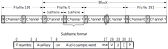
\includegraphics[height=0.25\textheight]{slides/audio-hardware/SPDIF.pdf}\\
  \end{center}
\end{frame}

\subsection{Auxiliary devices}

\begin{frame}{Auxiliary devices}
  \begin{itemize}
  \item Some devices may be on the analog path of the audio signal.
  \item They can be amplifiers, potentiometers or multiplexers.
  \item Some can be controlled and should be exposed as controls of
    the sound card.
  \end{itemize}
\end{frame}

\subsection{Clocks}

\begin{frame}{Clocks: producer/consumer}
  \begin{itemize}
  \item One of the DAI is responsible to generate the bit clock, it is
    the bit clock producer (previously: master).
  \item One of the DAI is responsible to generate the frame clock, it is
    the frame producer.
  \item Some CODECs have a great set of PLLs and dividers, allowing to get a
    precise BCLK from many different MCLK rates.
  \item Quite often, it is better to use the CODEC as producer. However,
    some SoCs have specialized audio PLLs.
  \end{itemize}
\end{frame}
